Another big part of the project involves Computer Vision, allowing the robot to detect and identify objects in the maze. The task is subdivided into smaller subtasks that are now discussed.

\subsection{Camera extrinsic calibration}
First, a camera extrinsic calibration is required in order to be able to express measurements in camera frame (\texttt{camera-link}) into the \texttt{world} frame. In this process, a 6 DoF transform is computed. Given that the transformation between \texttt{world} and \texttt{robot} is computed by the \texttt{odometry} node, it is natural to compute here the transformation between \texttt{robot} and \texttt{camera-link}. Then, it is easy to just use the \texttt{tf} package to transform between coordinate frames.

In this particular case, we only compute 4 out of the 6 DoF of the pose, since we assume the roll and yaw of the camera to be 0. Therefore, we only compute the pitch ($\phi$) and the translation vector $\textbf{t}$.\\
\textbf{Pitch}\\
To estimate the pitch, we first take the Point Cloud published by the PrimeSense camera and extract the main plane, corresponding to the floor. Then, the normal vector $\textbf{n}$ is computed. Finally, we extract the pitch of the camera from Equation \ref{eq:pitch}.

\begin{align}
\label{eq:pitch}
\phi = \cos^{-1}|n_y|
\end{align}

\textbf{Translation}
To compute the translation vector $\textbf{t} = \{t_x, t_y, t_z\}^T$, we take into account the transformation equation \ref{eq:homogeneous} in homogeneous coordinates:
\begin{align}
\label{eq:homogeneous}
\tilde{\textbf{p}}^R = T_{R}^{C} \tilde{\textbf{p}^C}
\implies
\begin{pmatrix}
x^R \\
y^R \\
z^R \\
1
\end{pmatrix}
=
\begin{pmatrix}
R & \textbf{t}\\
\textbf{0} & 1
\end{pmatrix} \begin{pmatrix}
x^C \\
y^C \\
z^C \\
1
\end{pmatrix}
\end{align}

, where $\textbf{p}_R$ and $\textbf{p}_C$ are a 3D point in robot and camera coordinate frames, respectively, $T_R^C$ is the transformation between the robot and the camera frame, $R$ is the 3D rotation and $\textbf{t}$ is the translation vector. 

R is computed from the yaw($\theta$), pitch ($\phi$) and roll ($\psi$) angles:
\begin{align}
R = R(\theta) R(\phi) R(\psi) = 
\begin{pmatrix}
\cos(\phi) & 0 & \sin(\phi) \\
0 & 1 & 0 \\
-\sin(\phi) & 0 & \cos(\phi) \\
\end{pmatrix}
\end{align}
, since $\theta = \psi = 0$.

To compute the translation vector, we require only one known 3D point in robot coordinates that we try to transform into the camera coordinate frame. To do that, we use a "calibration sheet" as shown in Figure XXXXX.


We detect the four corners of the rectangle using a Fast Feature Detector from OpenCV and take the mass center as the known point. It is easy to extract the 3D coordinate by just getting it from the depth image. 
Finally, we compute the translation vector applying Equation \ref{eq:translation}.
\begin{align}
\label{eq:translation}
\textbf{t} = \textbf{p}^R - R \textbf{p}^C
\end{align}

This concludes the calibration, which provides a transformation from \texttt{robot} frame to \texttt{camera-link} frame, and is published to the \texttt{tf} tree afterwards. 

\subsubsection{Tilt compensation}
Sometimes the robot tilts forward when braking and this greatly affect the calibration. Therefore, we implemented a small solution to fix this using the IMU. We basically compute the tilting of the robot ($\phi^R$) taking the measurements from the accelerometer, $a_x$ and $a_z$:
\begin{align}
\phi^R = \tan^{-1} \left(\frac{|a_x - a_{x0}|}{a_z}\right)
\end{align}

Since the construction is not perfect, we first calibrate the IMU by storing the initial tilt, measured by $a_{x0}$. 

Finally, the transformation between \texttt{robot} and \texttt{camera-link}, $T_0$, computed before, is corrected according to Equation \ref{eq:imu_tilt}.
\begin{align}
\label{eq:imu_tilt}
T' = T_{\text{IMU}} \cdot T_0 = 
\begin{pmatrix}
R(\phi^R) & \textbf{0}\\
\textbf{0} & 1 
\end{pmatrix} T_0
\end{align}

\subsection{Object detection}
The core of the computer vision component is divided into two modules. Object detection is mean to be fast (close to real-time computing time) and robust. Therefore, our aim was to optimize it as much as possible. The following pipeline was implemented.

\begin{enumerate}
\item First, we subscribe to the RGB and Depth images from the camera (for which we use the \texttt{ApproximateTime} and \texttt{Synchronizer} packages in ROS) and build a point cloud out of them. The reason for doing this is that for some reason the PrimeSense did not publish its own point cloud at a fixed rate, and it was quite far from 30 Hz (e.g.: every 200 ms or so), which was unacceptable. To make it faster, we downsampled the images by a factor of 4 in X and Y. For transforming points from 2D to 3D, we reverted the projection equation, as shown in Equation \ref{eq:2dto3d}.

\begin{align}
\label{eq:2dto3d}
X = z\cdot\frac{u - c_x}{f_x} \quad ; \quad
Y = z\cdot\frac{v - c_y}{f_y} \quad ; \quad 
Z = z
\end{align}

where $\{X,Y,Z\}$ is the 3D point in \texttt{camera-link} frame, $\{u,v\}$ is the 2D point from the RGB image, $z$ is the depth at the given point, and $c_x, c_y, f_x, f_y$ are the camera intrinsics, which are obtained from the \texttt{CameraInfo} message. 

\item We transform the point cloud into the \texttt{robot} coordinate frame and extract the floor as a separate point cloud. This is done using a simple \texttt{PassThrough} filter, preserving the points whose \texttt{z} component is smaller than 0.01 m. We could have used the \texttt{Plane Segmentation} library from PCL, but this was more computationally expensive and would not always work since it would remove only the dominant plane, which might not be always the floor.

\item A binary mask is created representing the floor by just reprojecting the floor point cloud extracted before. The process is done simply by reverting Equation \ref{eq:2dto3d} and getting $u$ and $v$. Since a subsampling was done at the beginning, it was necessary to apply dilation in order to have a solid mask.

\item Next, the floor is removed from the original RGB image by an AND operation with the negated floor mask. Now it that the yellow floor will not trigger false positives, it is possible to perform \textbf{color filtering}. We select to do this in the HSV color space given its better robustness against illumination. This is performed using a bank of 5 color filters (red, green, blue, yellow, purple) with ranges in H and S manually tuned for the application. The function \texttt{inRange} of OpenCV is used to quickly perform this filtering. The result is a set of binary masks, from which we select the one with a larger color response. After that, we find contours and filter them by size (a minimum is required) and the aspect ratio (a maximum value of 2 is used). 

If a contour still remains, it is likely that it belongs to an object. The biggest contour that fulfill these conditions is taken and a binary mask is created out of it using the \texttt{drawContours} function.

\item In case a contour belonging to a coloured object was found, we compute the 3D position of its mass center both in robot and world coordinates. If the object has not been recognized yet, and if it is close enough to the robot (less than 30 cm from it), the recognition module is called.

\end{enumerate}
Figure \ref{fig:detection} shows the process.

\begin{figure}[h]
        \centering
        \begin{subfigure}[b]{0.3\linewidth}
                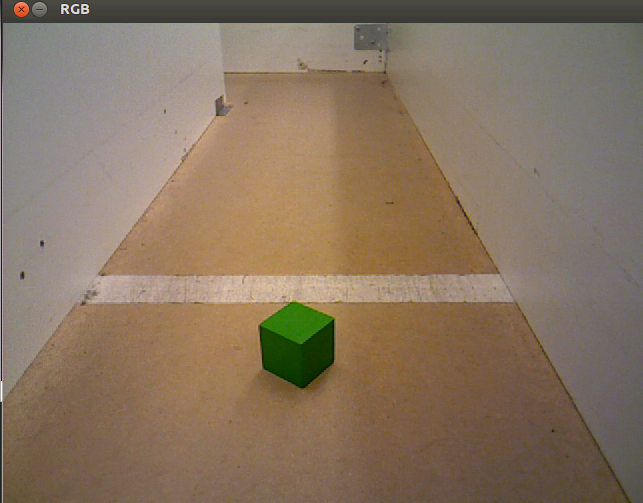
\includegraphics[height=3cm]{figures/RGB.png}
                \subcaption{Original RGB image}
        \end{subfigure}
        \begin{subfigure}[b]{0.3\linewidth}
                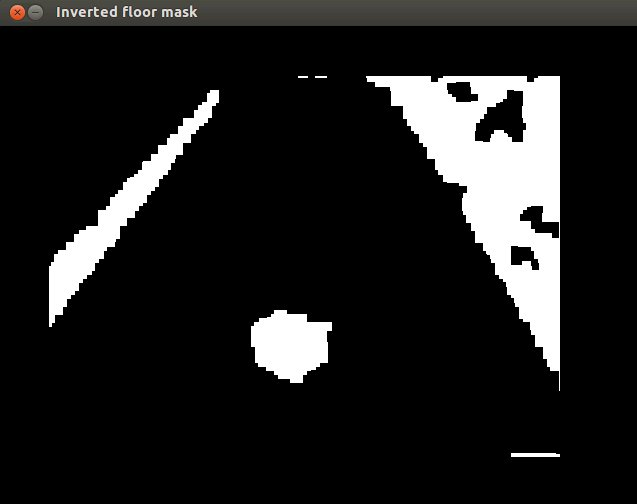
\includegraphics[height=3cm]{figures/no_floor_mask.jpg}
                \caption{Inverse of the floor mask}
        \end{subfigure}
        \begin{subfigure}[b]{0.3\linewidth}
                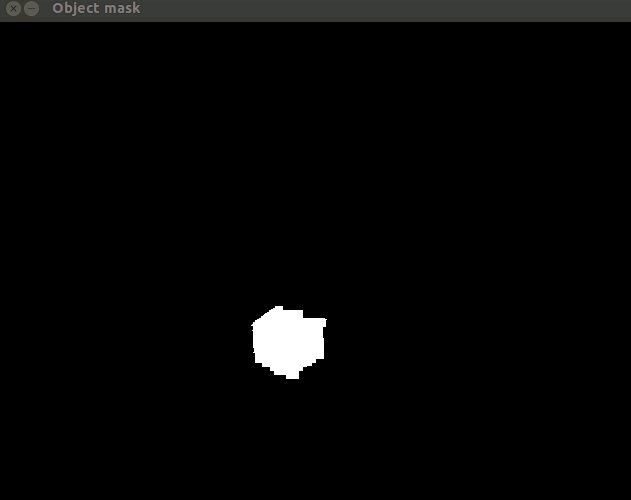
\includegraphics[height=3cm]{figures/object_mask.jpg}
                \caption{Object mask}
        \end{subfigure}
        \caption{Detection process}
        \label{fig:detection}
\end{figure}

\subsection{Object recognition}
A different number of approaches for object recognition have been tried. We decided to have a parallel research in both 2D and 3D methods for object recognition to analyze their advantages and disadvantages. 

\subsubsection{3D object recognition}
First, several attempts to perform 3D recognition were tried. We started using \textbf{feature matching} object recognition. The first question to ask was: what features? The task objects were too simple and had not texture, and therefore no keypoints could be extracted from them. Therefore, we tried to just subsample the point cloud to see if those points could act as keypoints.

Then, we tried several feature descriptors. We started with SHOT and PFHRGB, which were proven to provide a great accuracy (XXXXX REF). They did work well for cubes and balls, but we sadly discovered that it was not possible to do that with the hollow objects: they became "invisible" to the PrimeSense due to interferences with the IR projection, as can be seen on Figure \ref{fig:invisible}: 

\begin{figure}[h]
\centering
                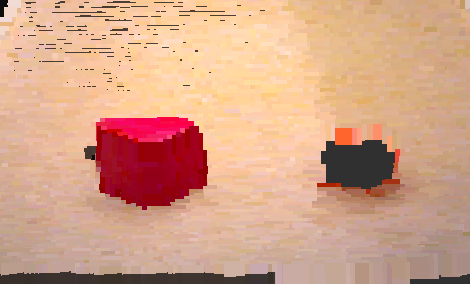
\includegraphics[height=3cm]{figures/concave.png}
                \subcaption{Red cube and "invisible" Patric}
		        \label{fig:invisible}
\end{figure}

The computational time was also quite expensive (around 1-2 seconds), and it was not robust against illumination since it was using RGB data. We further tried shape-only descriptors (PFH and FPFH) without a significant increase in performance. Therefore we abandoned the idea of 3D-only recognition.

\subsubsection{2D object recognition}
The "2D vision" refers to object recognition using only the RBG image from the camera as input and ignore the depth information, 2D vision returns a belief in terms of probability (0\%-100\%) of which object it thinks is in the input image (85\% red cube, 13\% yellow ball for example). The 2D vision basically combines color information with shape information of an object for identification. The 2D vision was coded, tested and implemented to the robot but was not used during the context due to worse performance compared with 3D object recognition.

The 2D vision contains 3 functions, one for circle recognition, one for triangle recognition and one for square recognition. The circles recognition function uses OpenCV built-in "Circle Hough Transform" method to find circular objects in an image. The triangle  and square recognition functions perform contour analysis to identify a triangle or a square in an image by analysing the number of lines in the contours and their crossing angles (for example a square always has 4 lines and 90 degrees between the lines). 2D vision also needed to perform some image transformations to the raw input RGB image before running the recognition algorithms to reach better performance and robustness, these transformations include resize/rescale of the original image, transforming RGB image into gray-scale image, Gaussian smoothing filter, Canny method to find contours in an image and finally dilate and erode images to remove single pixel objects and fill empty holes. See Figures \ref{fig:ryan1} and \ref{fig:ryan2}.

\begin{figure}[h]
        \centering
        \begin{subfigure}[b]{0.4\linewidth}
                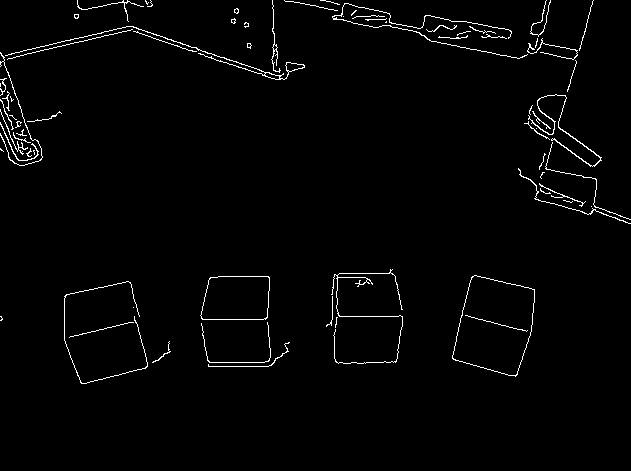
\includegraphics[height=4cm]{figures/canny.jpg}
                \subcaption{Canny method to find lines and contours.}
                \label{fig:ryan1}
        \end{subfigure}
        \begin{subfigure}[b]{0.4\linewidth}
                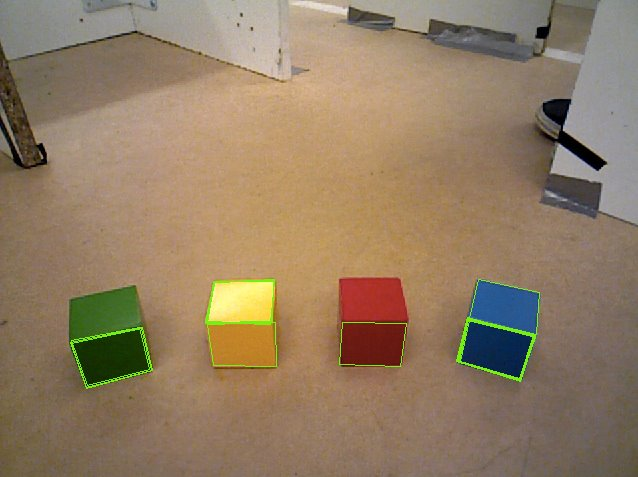
\includegraphics[height=4cm]{figures/squares.jpg}
                \caption{Found squares}
                \label{fig:ryan2}
        \end{subfigure}
        \caption{2D recognition example: square detection.}
\end{figure}

2D vision is perhaps the most "natural way" of how a robot can recognize objects, just like we humans, when we see an object we check out the color and the shape of the object and then decide/analyse what the object is. Unfortunately many problems can occur even in such a "controlled" environment such as the maze that makes the 2D vision very hard to be 100\% robust. Different light condition in the environment (due to weather, lamp, shadow etc), different rotation of how the object is placed in front of the camera, and noise from the camera and the environment (robot vibration, tape on the walls etc) can all make the 2D vision perform worse than expected. Resize/rescale the raw image was a method used to successfully reduce execution time of the algorithm; it could also be used to remove noise from the image. Another way to reduce image noise is Gaussian smoothing, however it also removes useful information such as object contours if the parameters are not chosen carefully, the same problems apply to dilate and erode method, essentially it is always a trade-off between removing unnecessary information and keeping useful information. Canny method was used for finding lines and contours in an image, it works best on gray-scale image so we must convert all image to gray-scale image. When converting an RGB image into a gray-scale image, if you already knew for example that the object being recognized is red, one smart way of doing it is to just split the RGB image into 3 channels and choose the R channel as your gray-scale image, this way most of the red contours are being saved compared with the normal OpenCV "RGB2GRAY" function. An attempt to fight against different light condition was to multiply the raw RGB image with different constants such as from 0.8 (to make the image darker) and 1.5 (to make the image brighter) with 0.1 intervals. This method greatly improved the recognition rate and made sure that at least the object will be detected in one or two light constants. However misdetection problem also followed and it also caused problem for calculating the probability of recognizing an object.

Text below the images:
Fig1: 
Fig2: .
\subsubsection{Final approach}
The final approach was to determine a \textbf{probabilistic formulation} of the problem in order to gain in robustness and be able to reason about the certainty of the recognition. The most likely object $o^*$ was determined using a MAP estimate given the measurements in 3D shape $z^s$ and color $z^c$, according to Equation \ref{eq:obj_map}.

\begin{align}
\label{eq:obj_map}
o^* = \arg\max_o p(o|z^s, z^c) = \arg\max_o \eta p(z^s, z^c|o) p(o) = \arg\max_o p(z^s|o)p(z^c|o)
\end{align}

Here we are assuming that all the objects have the same prior probabilities and that the shape and color are conditionally independent given the object. 
We now describe the way to compute the previous probabilities.

\textbf{3D shape probability}
For the task of 3D shape recognition, we make use of the VFH descriptor included in the PCL library. Unlike the previously described descriptors (FPFH, PFHRGB,...), this is a \textbf{global} descriptor, which means it does not have to be applied to all possible keypoints of the object, but rather it is applied to the whole point cloud. It is rotation and scale invariant, which is important for the application. 

We build a 3D model database for the objects. We realized early in the course that \textbf{hollow objects} are invisible to the PrimeSense due to interference generated by the IR projector. Therefore, we only built 3D models for the ball and cube. 50 models were taken for each of them at different distances from the camera and with different poses. 

After that, the test point cloud (which contains a potential object) is matched against the database. This is done quickly by histogram matching, for which OpenCV has some metrics. We opted for using the \textbf{correlation} metric between histograms. W

A value of -1 means complete opposite correlation, while 1 means perfect match. Therefore, we compute the probability of 3D shape as follows:
\begin{align}
p(z^s = \text{cube} | o) = \max_i 0.5\cdot(d(H_{\text{test}}, H_{\text{cube}}^i) + 1.0) \\
p(z^s = \text{ball} | o) = \max_i 0.5\cdot(d(H_{\text{test}}, H_{\text{ball}}^i) + 1.0) \\
\end{align}

where $H_{\text{cube}}^i$ and $H_{\text{ball}}^i$ are the descriptors of the 3D models from the database.

\textbf{Hollow probability}\\
We also take into account the probability that an object is hollow, according to Equation \ref{eq:probHollow}.
\begin{align}
\label{eq:probHollow}
p(z^s = \text{other} | o) = 1.0 - N_d/N_T
\end{align}

, where $N_d$ is the number of pixels inside the object mask that have a valid (non-zero, not NaN) depth and $N_c$ is the number of pixels within the object mask.

These three probabilities are normalized afterwards so that they add up to 1.

\textbf{Color probability}\\
In this task, it is not possible to recognize all the objects without color information. For this we implemented a Bayes Classifier XXXX ref on the HSV color model. We currently only use the H and S components, which influence most the outcome. 

The first step is to create a \textbf{color model}. We decided to have independent Gaussian distributions for 7 colors (red, green, blue, yellow, purple, orange, light green) and for each of the channels (H and S), so the total number of parameters is $7 \cdot 2 \cdot 2$ = 28. For every color, the model ${\mu_h, \sigma_h, mu_s, \sigma_s}$ is computed from training data. In particular, 50 pictures from each of the 10 objects were taken at different positions and different light conditions. In sum, 500 pictures form the color model. An application was implemented in order to speed up the capture of data. In particular, the application would cut out an image from a predefined region of interested at a fixed rate (e.g.: every 5 seconds). Finally, the color model was computed by extracting the mean and variance values for each color and channel.

During the test phase, the Bayes Classifier was applied to every pixel included in the object mask to determine to which class it belonged to. Finally, the probability of any color is computed as follows:
\begin{align}
p(z^c = c | o ) = N_c / N_T
\end{align}

, where $N_c$ is the number of pixels belonging to class $c$, and $N_T$ is the total number of pixels in the object mask. 

\subsection{Obstacle detection}

In addition to the so-called "IR bumper" (see section XXXXXXXXXXXXX), an obstacle avoidance solution using the PrimeSense camera was implemented. The aim was to detect also objects right in front of the robot, especially the edge of walls that would not be detected by the front IR sensor.

To do this, we simulated a laser scanner using the depth image. The implemented pipeline is as follows:

\begin{enumerate}
\item Build a point cloud from the depth image and transform it into the \texttt{robot} coordinate frame. Here color was not required. 
\item Filter the point cloud to determine the working region. In particular, the 3D points following these constraints were selected:
\begin{itemize}
\item $0.2 < x < 0.4$
\item $-0.115 < y < 0.115 $
\item $0.05 < z < 0.06$
\end{itemize}

All the values are expressed in meters. In other words, a thin slice (0.01 m thick) covering an area of a width equals to the robot width (23 cm) and a maximum depth of 0.4 m (from the center of the robot).

\item Simulate laser beams. For this, the previous point cloud was filtered multiple times (once per line) using the constraint: $ i < y < i+0.005$, for $i = -0.115, \dots, 0.115$, increasing in steps of 0.005 meters. That is: lines with 0.005m resolution where taken. 
\item Analyze the occupancy of the laser beam. This was done simply by checking if the previously filtered cloud lines contained any point. In that case, information about the minimum depth at which there was a point in the cloud was obtained.
\end{enumerate}

The result of the algorithm is a set of lines in the forward direction of the robot that determine the occupancy of the region in front of it. An example is shown in Figure \ref{fig:laser}
\begin{figure}[h]
        \centering
        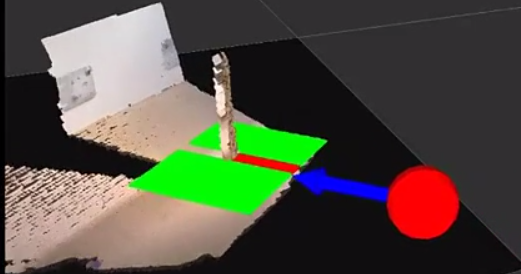
\includegraphics[height=4cm]{figures/laser.png}
        \caption{Simulated laser scanner detecting thin wall.}
        \label{fig:laser}
\end{figure}

This information is afterwards sent to the \texttt{mapping} node, which sets to \emph{blocked} the cells corresponding to the end point of the lines of the laser scan that do not show free space. 
